\chapter{Marco Teórico}
\label{teorico}

\section{Adquisición de imágenes de rayos X}

La obtención de una imagen radiográfica es el resultado de una compleja cadena de procesos
físicos que comienza con la generación controlada de fotones de alta energía y culmina en la
transformación de estos en señales eléctricas digitales. Para comprender la naturaleza de la
información contenida en una microtomografía, es imperativo analizar primero la física detrás
de la formación de la imagen. Esto implica descomponer el proceso en sus tres pilares fundamentales:
la generación del haz en la fuente de emisión, los mecanismos de interacción radiación-materia
que ocurren en el interior del volumen y la respuesta del sistema de detección digital. Estos
procesos determinan tanto el contraste como la resolución espacial final, estableciendo el
límite teórico de lo que el sistema es capaz de resolver.


\subsection{Interacción de la radiación con la materia}

Los rayos X son una forma de radiación electromagnética de alta energía, con
longitudes de onda entre 10 nm y 10 pm, aproximadamente. Sin embargo, en el 
contexto de este trabajo, es más conveniente 
estudiar su comportamiento corpuscular: los fotones. Al atravesar un material,
estos pueden interactuar con las moléculas, átomos, núcleos o electrones que la
componen. Las interacciones pueden ser dispersiones elásticas o inelásticas,
donde el fotón se dispersa conservando o perdiendo su energía, respectivamente, o
de absorción total, en la que el fotón es completamente absorbido por el blanco.
Dichas interacciones tienen distintas probabilidades de ocurrencia, que dependen
de la energía del fotón incidente ($\sim$0.1-200 keV en el caso de rayos X), y de
características del material, como densidad, número atómico, capas electrónicas,
etc. Para las energías de rayos X, las interacciones más probables son efecto fotoeléctrico (absorción total),
efecto Compton (dispersión inelástica con electrones) y dispersión Rayleigh
(dispersión elástica con electrones). \cite{Als-Nielsen2011}

Cuando un haz de rayos X atraviesa un medio material, los fotones que lo
componen irán interactuando con la materia de alguna de las formas antes
mencionadas con sus respectivas probabilidades (como se observa en la figura
\ref{fig:interacciones}). Observando el haz 
en su totalidad, esto se traduce en una atenuación
del mismo, cuya magnitud depende de la energía del haz, la cantidad de materia 
atravesada y las características propias del material. En otras palabras, si
inciden $n$ fotones por unidad de área y unidad de tiempo sobre una lámina de
espesor $\Delta x$ y $n'$ es el número de fotones que salen ($n'<n$), se observa
experimentalmente que la fracción de fotones atenuados por un determinado efecto $i$
es proporcional al espesor. Es decir, si $\Delta n = n' - n$, entonces se tiene que

\begin{equation}
    \left(\frac{\Delta n}{n}\right)_i = -\gamma_i \Delta x
    \label{eq:atenuacion1}
\end{equation}

\noindent donde $\gamma_i = \gamma_i(E,Z)$ es el coeficiente de atenuación lineal correspondiente
al efecto $i$, que depende de la energía $E$ del haz y el número atómico $Z$ del 
material. Cada interacción tiene un coeficiente de atenuación lineal asociado ($\sigma$: Compton;
$\tau$: fotoeléctrico; $\sigma_R$: Rayleigh), y este está relacionado con la probabilidad
de que un fotón interactúe de esa forma. \cite{Als-Nielsen2011}

Se considera que cada proceso de
atenuación afecta a la radiación incidente en forma independiente de los otros,
por lo tanto, al estudiar todos los efectos en conjunto en un haz, se tiene que

\begin{equation}
    \frac{\Delta n}{n} = -\mu \Delta x, \hspace{5mm} \mu = \sum_{i} \gamma_i \hspace{5mm},
    \label{eq:aten_tot}
\end{equation}

\noindent donde $\mu$ es el coeficiente de atenuación lineal total. Llevando al límite de 
espesor muy pequeño, se tiene que $\Delta x \rightarrow dx$, $\Delta n \rightarrow dn$, e integrando, se obtiene

\begin{equation}
    n = n_0 e^{-\mu x} \hspace{5mm},
    \label{eq:atenuacion}
\end{equation}

\noindent donde $n_0$ es el número de fotones incidentes sobre la lámina, por unidad de
tiempo y unidad de área, y $n$ es el número de fotones resultantes tras haber
atravesado un espesor $x$ del material (en el resto del trabajo, se hablará de la
intensidad del haz $I$ en vez del número de fotones, ya que ambas cantidades son
equivalentes). \cite{Als-Nielsen2011}

\begin{figure}[htpb]
    \centering
    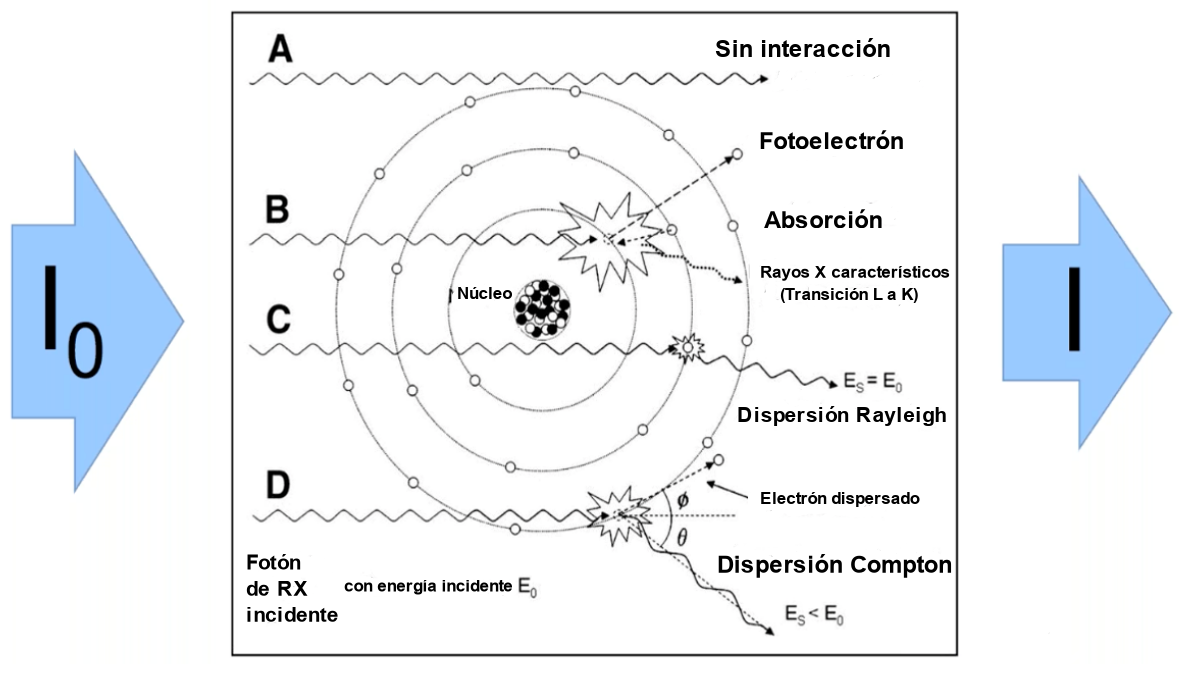
\includegraphics[width=0.6\textwidth]{images/interacciones.png}
    \caption{Posibles interacciones de fotones de rayos X (energías entre 0.1 y 200 keV), ya
    sea con electrones externos, internos o con núcleos.}
    \label{fig:interacciones}
\end{figure}

Si el blanco atenuador está compuesto por $N$ elementos en concentraciones másicas
dadas por $C_i = m_i/\sum_{i=1}^{N}m_i$ (con $m_i$ la masa del elemento $i$),
se puede considerar que el espesor $\Delta x$ está compuesto por distintas capas
de espesores $\Delta x_i$, correspondientes a cada elemento, para obtener un $\mu$
total de la forma

\begin{equation}
    \mu = \rho \sum_{i=1}^{N} \frac{\mu_i}{\rho_i} C_i
    \label{eq:mu_total}
\end{equation}

Por otro lado, la ecuación \ref{eq:atenuacion} es válida solo para un haz monocromático,
es decir, con una única energía $E$ en todos sus fotones. Sin embargo, en la mayoría
de los casos (sobre todo en la adquisición de radiografías), se suele trabajar con un
haz policromático con una distribución de energía $I_0(E)$ incidente. De esta forma, cada
fotón se atenuará con una proporción distinta, en función de $\mu(E)$, obteniéndose
que la intensidad resultante del haz tras atravesar un espesor $t$ es

\begin{equation}
    I = \int I_0(E) e^{-\mu(E,Z)t} dE
    \label{eq:policrom}
\end{equation} \cite{Als-Nielsen2011}

En general, se observa experimentalmente que $\mu(E,Z)$ disminuye cuando la energía
$E$ del haz aumenta (siendo
$Z$ los elementos que componen la muestra). Es decir, mientras más energía tengan los fotones, menor es
la probabilidad de que ocurra alguna interacción con la materia que atraviesan,
como se observa en la figura \ref{fig:coef_abs_agua}, para el agua.

\begin{figure}[htpb]
    \centering
    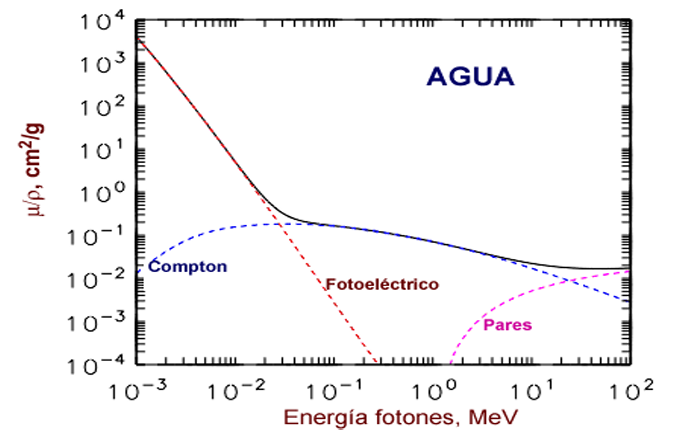
\includegraphics[width=0.5\textwidth]{images/coef_abs_agua.png}
    \caption{Coeficiente de atenuación másico $\mu / \rho$ del agua, en función
    de la energía $E$ del haz incidente.}
    \label{fig:coef_abs_agua}
\end{figure}

\subsection{Imágenes Radiográficas}

El proceso de obtención de una radiografía consta de 3 partes: la producción del haz de
rayos X, la interacción con la muestra y la adquisición en sí de la imagen a través
de un detector. La producción del haz se realiza con una fuente de rayos X, un
dispositivo que contiene un ánodo y un cátodo inmersos en un vacío dentro de un tubo (fig. \ref{fig:fuente}.a). El cátodo tiene
en su extremo un filamento que emite electrones al calentarse por una corriente.
Dichos electrones son acelerados mediante un voltaje (del orden de kV) hacia el ánodo,
cuyo extremo suele ser de tungsteno o molibdeno. Al impactar los electrones contra este blanco,
se emiten rayos X característicos (propios del material del ánodo) y radiación de
frenado, que salen del tubo como un haz cónico al pasar por una ventana de
berilio (material que absorbe muy poco los rayos X). Debido a las interacciones
que participan en el proceso, el haz resultante es policromático, con una distribución
de energía continua y con los picos característicos correspondientes (ver figura
\ref{fig:fuente}.b). Cambiando
el voltaje, se puede modificar la energía media del haz, y controlando la corriente
aplicada se puede aumentar o disminuir la cantidad de fotones generados (es decir,
la intensidad).

\begin{figure}[htpb]
    \centering
    \begin{subfigure}{0.3\textwidth}
        \centering
        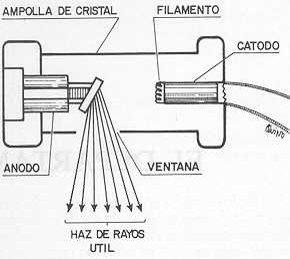
\includegraphics[width=\textwidth]{images/fuente_a.jpg}
        \caption{}
    \end{subfigure}
    \hspace{10mm}
    \begin{subfigure}{0.5\textwidth}
        \centering
        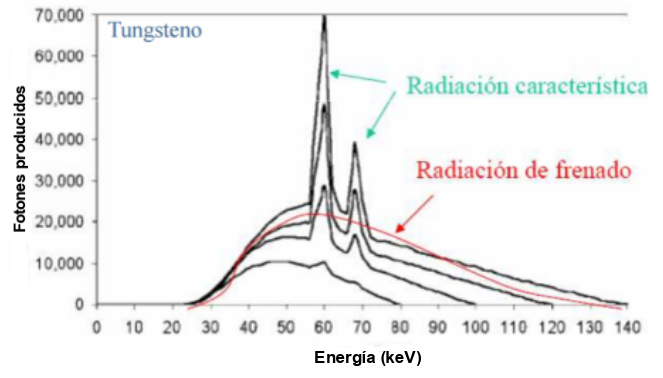
\includegraphics[width=\textwidth]{images/espectro_teorico.png}
        \caption{}
    \end{subfigure}
    \caption{Esquemas de producción de rayos X. (a) Se calienta el filamento a través
        de una corriente, emitiendo electrones que son acelerados hacia el ánodo a partir
        de una diferencia de potencial. Al impactar contra este, se generan rayos X por
        radiación de frenado y emisión de fotones característicos (b).}
    \label{fig:fuente}
\end{figure}

El haz obtenido sale de la fuente y atraviesa la muestra, ocurriendo en su interior
todas las interacciones mencionadas en la sección anterior (fig. \ref{fig:interacciones}). Así se va atenuando
hasta salir del objeto y alcanzar el detector digital. Este último registra la
cantidad de fotones que traspasaron la muestra sin interactuar a través de una
grilla cuadriculada de foto-diodos individuales (el tipo de detector de
pantalla plana más común) o una capa de un fotoconductor. Cada celda del detector produce una
señal eléctrica proporcional a la cantidad de fotones que reciben en un determinado
tiempo. Esto es interpretado digitalmente como pixeles con distintas tonalidades de gris. \cite{Stock2019}

En la figura \ref{fig:radiografia_mod} se puede observar con mayor detalle el proceso con
un esquema simplificado.
Un haz policromático de intensidad $I_0(E)$ interactúa con un volumen de espesor
$t$, en la posición $(x,y)$, con un coeficiente de atenuación $\mu(x,y;E,Z)$. Tras atenuarse, el haz que llega al
pixel $(x,y)$ del detector tiene una intensidad $I(x,y)$ dada por la ecuación $\ref{eq:policrom}$.
\medskip
\medskip

\begin{figure}[htpb]
    \centering
    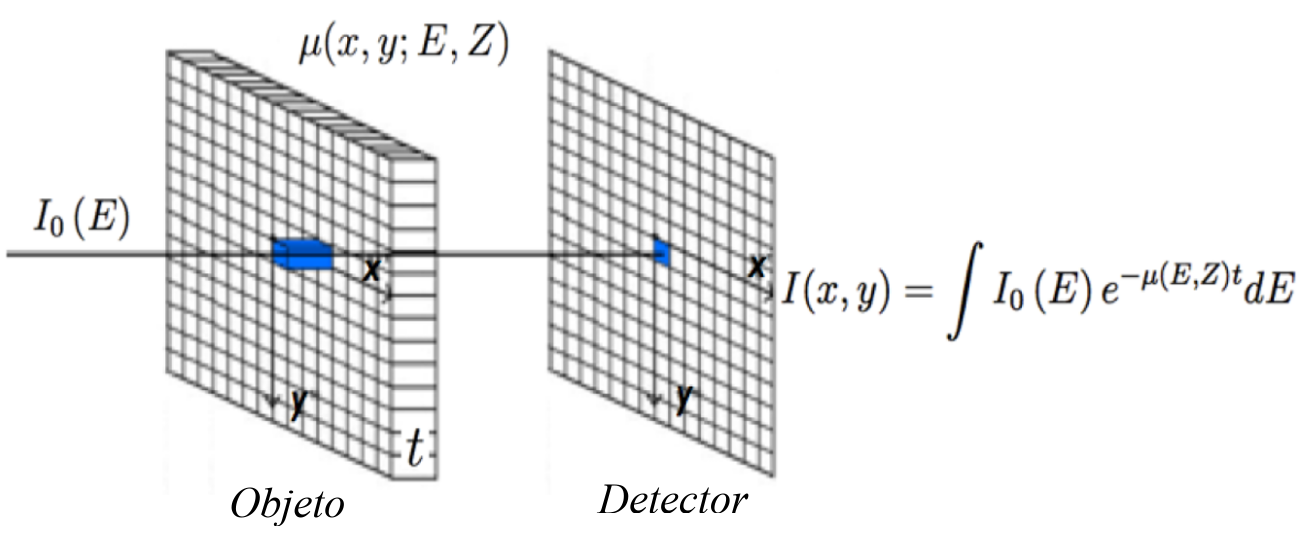
\includegraphics[width=0.6\textwidth]{images/radiografia_mod.png}
    \caption{Esquema simplificado del proceso de adquisición de una radiografía. Un haz de rayos X con intensidad $I_0(E)$
    atraviesa un volumen de espesor $t$ y coeficiente de absorción $\mu(x,y;E,Z)$. Tras interactuar
    con la materia, se atenúa y llega al pixel $(x,y)$ del detector con una intensidad $I(x,y)$.}
    \label{fig:radiografia_mod}
\end{figure}

Como puede observarse en la figura \ref{fig:radiografia_mod}, cada pixel de la imagen
obtenida, se asocia a un volumen (voxel) de la muestra, de las mismas dimensiones
en la sección transversal y de espesor $t$. Las diferencias de intensidad detectada,
o el ``contraste'' que se observa en la imagen, es el resultado de las variaciones
del coeficiente de atenuación en la muestra y/o las variaciones de espesor. Por lo
tanto, se define el \textit{contraste} en la imagen como la cantidad $\mu(E,Z)\cdot t$.
De esta forma, se puede obtener información de la estructura interna de una muestra
de composición variada y con distintos espesores, por ejemplo la mano de la figura
\ref{fig:radiografia_mano}, que contiene tejido duro, (hueso), y tejido blando
(músculo, piel, etc.). Sin embargo, la información que se puede extraer de una
radiografía es limitada por esta razón: sin un conocimiento previo de la muestra,
es imposible determinar solo el espesor $t$ o solo el coeficiente $\mu(E,Z)$,
y dos pixeles podrían tener la misma tonalidad de gris (contraste), y tener valores de
$t$ y $\mu$ completamente distintos. Así, se puede definir una radiografía como
una \textit{proyección de $\mu$ en la dirección del haz} sobre el plano del detector.

\begin{figure}[htpb]
    \centering
    \begin{subfigure}{0.24\textwidth}
        \centering
        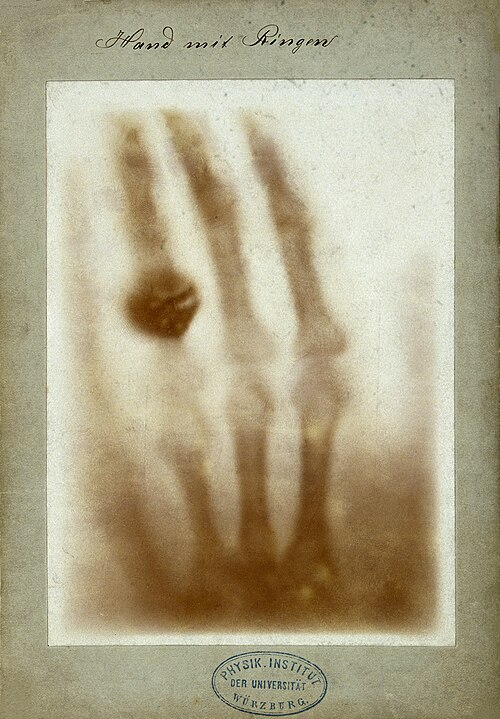
\includegraphics[width=\textwidth]{images/first_radiog.jpg}
    \end{subfigure}
    \hspace{10mm}
    %\hfill
    \begin{subfigure}{0.31\textwidth}
        \centering
        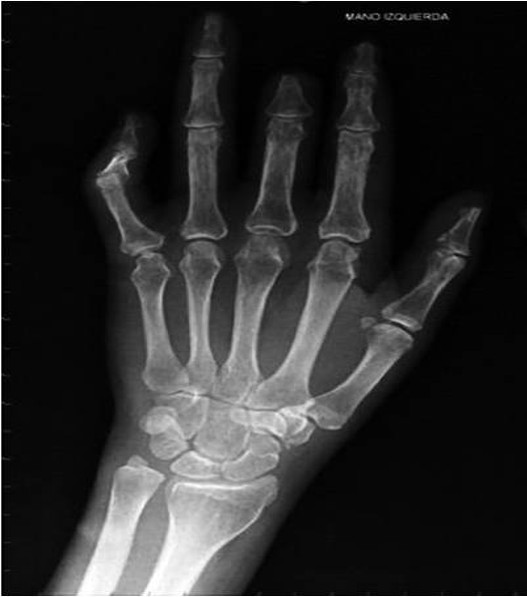
\includegraphics[width=\textwidth]{images/radiografia_mano.jpg}
    \end{subfigure}
    \caption{Primera radiografía de la historia, obtenida por W.C. Röntgen en 1895, de
    la mano de su esposa (izq.). Radiografía moderna de una mano humana (der.).}
    \label{fig:radiografia_mano}
\end{figure}

\subsection{Imágenes tomográficas}

Una tomografía es un \textit{mapa tridimensional del coeficiente de absorción $\mu$
de la muestra}, por lo que está exenta de las limitaciones propias de las
radiografías. Sin embargo, su adquisición requiere la obtención de múltiples
imágenes radiográficas de la muestra, llamadas proyecciones, en distintas direcciones
(realizando un barrido angular de $180^{\circ}$ o 360$^{\circ}$, con una distancia angular
constante entre cada imagen). Luego, la reconstrucción tomográfica se realiza por
cortes o \textit{slices} en el plano perpendicular al eje de rotación (eje $z$ de
la muestra), tal que para cada altura $z$ se toma la información de todas las proyecciones
y se procesan para obtener una imagen del coeficiente $\mu(x,y)$.

Por último, se agrupan todas las \textit{slices} reconstruidas y se ``apilan'' para formar
un mapa tridimensional del coeficiente de absorción $\mu(x,y,z)$, representado por
un valor numérico (un tono de gris) correspondiente al voxel $(x:x+\Delta x, y:
y+\Delta y, z:z+\Delta z)$, y que puede visualizarse como un modelo 3D mediante
algún software especializado.

La reconstrucción tomográfica es posible a partir de los teoremas y la transformada
de Radon, introducidas en 1917 por el matemático J. Radon. Se define la transformada
bidimensional de Radon de la función $f(x,y)$ como

\begin{equation}
    p(\xi, \gamma) = R_2 \{f(x,y)\} = \int f(\xi,\eta)d\eta
    \label{eq:transformada_radon}
\end{equation}

\noindent donde para cada ángulo $\gamma$ se definen los ejes perpendiculares $\xi$ y $\eta$,
y para cada coordenada $\xi$ se realiza la integral de línea en la dirección
de $\eta$, como se muestra en la figura \ref{fig:transf_radon}. Por otro lado,
el teorema de Radon afirma que \textit{su transformada es invertible.} Es decir
se puede reconstruir la función $f(x,y)$ a partir de su transformada. \cite{Als-Nielsen2011}

\begin{figure}[htpb]
    \centering
    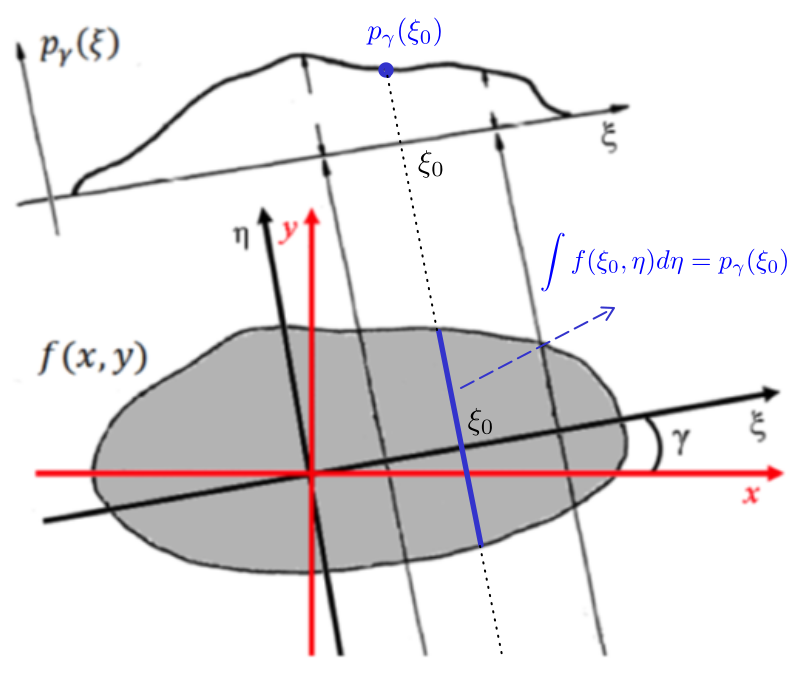
\includegraphics[width=0.5\textwidth]{images/transf_radon.png}
    \caption{Esquema de la transformada de Radon. Para cada ángulo $\gamma$ entre 
    el eje $x$ y un eje $\xi$, se obtiene una proyección $p_\gamma(\xi)$, que 
    es la integral de línea de $f(x,y)$ en la dirección $\eta$ (perpendicular a $\xi$).
    En el caso de una tomografía, la dirección $\eta$ es la dirección del haz de rayos X
    paralelos que atraviesan la muestra para una proyección específica.}
    \label{fig:transf_radon}
\end{figure}

Si se considera un haz monocromático que atraviesa una muestra (con $\mu(x,y)$
variable en el espesor), en una dirección perpendicular al eje $\xi$ (coplanar
con $x$ e $y$), entonces la proyección radiográfica de un solo corte transversal
es una línea de pixeles \{px$_1$, px$_2$, ..., px$_{\xi}$\} con intensidades $I(\xi)$ dadas por la ecuación

\begin{equation}
    I(\xi) =  I_0(\xi)e^{-\int \mu(\xi,\eta)d\eta}
    \label{eq:proyeccion}
\end{equation}

\noindent donde la integral se realiza sobre el espesor atravesado en la dirección del haz.
De esta forma, podemos despejar y obtener la transformada de Radon de $\mu(x,y)$.

\begin{equation}
    -ln\left(\frac{I(\xi, \gamma)}{I_0}\right) = \int \mu(\xi,\eta)d\eta = R_2\{\mu(x,y)\}
    \label{eq:transf_mu}
\end{equation}

Así, se puede medir el parámetro $\ln(I(\xi, \gamma)/I_0)$ (para todos los ángulos $\gamma$) y anti-transformarlo para
obtener el mapa bidimensional de $\mu(x,y)$ para ese plano. Repitiendo el proceso
para todos los planos en $z$, se obtiene una reconstrucción tomográfica completa.
La necesidad de múltiples proyecciones, en distintos ángulos, radica en que la
transformada de Radon de $\mu(x,y)$ es una función $p(\xi,\gamma)$, con $\gamma$
el ángulo de la proyección (fig. \ref{fig:transf_radon}). \cite{Als-Nielsen2011}

% Para la representación de los resultados es común utilizar las unidades de Hounsfield
% ($HU$), donde se relaciona el coeficiente de absorción $\mu$ del material con el
% del agua ($\mu_{agua}$).

% \begin{equation}
%     HU = \dfrac{\mu - \mu_{agua}}{\mu_{agua}}
%     \label{eq:HU}
% \end{equation}

El teorema de Radon es la demostración matemática y el fundamento detrás de la reconstrucción
tomográfica a partir de proyecciones, sin embargo, calcular la anti-trans\-for\-ma\-da
del logaritmo explicítamente no es algo trivial, y generalmente implica un alto
costo computacional. Para ello, se han implementado distintos métodos y aproximaciones
que facilitan la tarea. Entre ellos, el más usado y extendido, por ser rápido,
sencillo y eficiente, es el algoritmo de \textit{Retro-proyección filtrada}. Este
funciona siempre y cuando la intensidad transmitida (el número de cuentas) sea 
alta, algo usual en la mayoría de tomografías de rayos X. \cite{Stock2019}\cite{Als-Nielsen2011}

Por otro lado, la transformada de Radon es una función $p(\xi,\gamma)$ que depende del ángulo
$\gamma$ de la proyección, como se mencionó antes, y esto implica la necesidad de múltiples
proyecciones. Lo mismo sucede para cualquier algoritmo de reconstrucción.
El mínimo número de proyecciones (MNP), está dado por el \textit{Teorema de muestreo
de Nyquist-Shanon} \cite{Nyquist}, el cual dice que para mantener la resolución del detector, haciendo
un barrido de 180$^{\circ}$, el MNP debe ser igual al número de pixeles que ocupa el ancho
(perpendicular al eje de rotación) de la región de interés en la imagen.

\subsection{Micro-radiografía y micro-tomografía}

Las figuras \ref{fig:radiografia_mod} y \ref{fig:transf_radon} son válidas cuando
los rayos X incidentes son paralelos entre sí. Sin embargo, debido al diseño de
las fuentes más comúnmente usadas, esto no suele ser la norma en los tomógrafos, sino que se suele trabajar
con haces cónicos o haces de tipo abanico (similar al cónico, pero los rayos solo
se propagan en un mismo plano) cuyo foco es la sección del ánodo, de la que se emiten los fotones.
Si la región de interés es muy pequeña y se encuentra
en el área central del cono/abanico, entonces los rayos pueden aproximarse como
paralelos, pero incluso si este no es el caso, los métodos de la anti-transformada
de Radon y la retro-proyección filtrada pueden adaptarse sin mucha dificultad a
la geometría. Pero la utilidad de un haz cónico va más allá del diseño de la fuente,
y es la posibilidad de realizar una magnificación de la imagen, permitiendo explorar
detalles muy pequeños de la muestra, con alta resolución espacial. Los avances
tecnológicos han permitido diseñar microtomógrafos capaces de detectar detalles
del orden 1 $\mu$m, e incluso, centenas de nm (llamados ``nanotomógrafos'' \cite{Claro2023}).

El fundamento detrás de esto está en el tratamiento de los rayos X emitidos, bajo la
óptica geométrica, teniendo en cuenta que, a diferencia de la luz visible, los rayos X no proyectan sombras opacas debido a
su capacidad de atravesar la materia. Así, se define la magnificación $M$ de un sistema
de micro-tomografía como

\begin{equation}
    M = \frac{\Delta x_{proy}}{\Delta x_{real}} = \frac{D}{F}
    \label{eq:magnificacion}
\end{equation}

\noindent donde $\Delta x_{real}$ es una distancia en alguna dirección (arbitraria, pero en un
plano paralelo al detector) de la muestra, y $\Delta x_{proy}$ es la distancia correspondiente
a $\Delta x_{real}$ que se proyecta directamente sobre el detector para obtener
una imagen radiográfica. Por otro lado, $D$ y $F$ son las distancias fuente-detector
y fuente-objeto respectivamente, de acuerdo con las consideraciones de la óptica geométrica.

Se entiende por \textit{resolución espacial} ($RE$) a la distancia mínima entre dos elementos de la muestra
que al proyectarse sobre el detector (o al reconstruirse, si hablamos de tomografía),
pueden distinguirse como elementos distintos. También suele medirse desde el dominio de
las frecuencias espaciales, como lp/mm (``pares de línea por milímetro'') o ciclos/mm,
es decir, la cantidad de ciclos de una frecuencia espacial (por ejemplo, líneas blancas
y negras) que pueden distinguirse en una distancia determinada. En general, la resolución espacial de un microtomógrafo
está determinada por todos los procesos de ``transferencia'' de señal que ocurren en una
adquisición: desde la producción y colimación inicial de los rayos X, sus interacciones
con la muestra, su interacción con el centellador (si el detector tiene) e interacción con los foto-diodos, el proceso de transformación
a una señal eléctrica, la digitalización de esta misma, y el algoritmo de reconstrucción.

Cada uno de estos procesos altera la señal original y funciona como un ``filtro'' que
difumina los detalles de la muestra \cite{Buzug2008}. Sin embargo no todos tienen el mismo peso, y en
los microtomógrafos actuales, los factores más influyentes son la magnificación $M$ del
sistema, el tamaño del pixel $\Delta p$ del detector y el tamaño focal $S$ (diámetro del foco,
el área desde donde se emiten los rayos X).
Los primeros dos pueden entenderse a partir de la ecuación \ref{eq:magnificacion}, siendo
$\Delta p = M \Delta x_{min}$ la magnificación de la distancia mínima distinguible cuando
la fuente es puntual. Pero en realidad las fuentes no son puntuales, lo que implica también un
área de ``penumbra'' en los bordes. Luego, se utiliza la siguiente expresión como aproximación
de la resolución espacial de un microtomógrafo. \cite{JunYan2010}

\begin{equation}
    RE = \sqrt{\left(S\dfrac{M-1}{M}\right)^2 + \left(\frac{\Delta p}{M}\right)^2} 
    \hspace{10mm} [\text{lp/mm}] = \frac{1}{2\cdot RE[\text{mm}]} 
    \label{eq:res_espacial}
\end{equation}

\noindent donde el factor $1/2$ en la conversión a lp/mm está relacionado a la frecuencia de corte
o frecuencia de Nyquist, que es la frecuencia máxima que puede ser detectada por un 
sistema de muestreo \cite{Nyquist} \cite{Buzug2008}.

\subsection{Artefactos}

Se define como artefacto de una radiografía/tomografía con toda distorsión de la imagen
que dificulte la visualización de las estructuras propias del objeto. Suelen
presentarse como rayas, ruido, alteraciones de la arquitectura, anillos, bandas
blancas y negras superpuestas, entre otros (ver figura \ref{fig:artefactos}); y 
tienen tres orígenes posibles: físico, cinético y técnico. A continuación se 
mencionarán algunos de los más pertinentes para este trabajo:

\begin{itemize}
    \item Volumen parcial (físico): si la muestra tiene un cambio de contraste brusco, un
    borde ``filoso'', este se digitalizará como un cambio lineal de intensidad en varios
    pixeles, efectivamente mostrando un borde borroso. Esto se debe a que las
    intensidades calculadas para cada pixel tienen cierta dependencia de los valores de
    sus vecinos, y también a los procesos de reconstrucción empleados. Además, otro factor
    en juego es el tamaño de foco de la fuente (que no es puntual), que genera un efecto
    de ``penumbra'' \cite{Buzug2008}.
    \item Endurecimiento del haz (físico): a menor energía, más probable es la
    interacción de un fotón con la materia, por lo tanto, cuando un haz policromático
    atraviesa un material, serán estos fotones los que sean absorbidos con más frecuencia.
    Así, la distribución de energía del haz incidente cambia capa a capa, y como $\mu(E)$
    depende de la energía, se medirá un $\mu$ menor al real, mientras mayor sea el
    espesor (incluso si el material es homogéneo y uniforme en toda la muestra) \cite{Buzug2008}.
    \item Baja tasa de conteo (físico): si la muestra es de gran espesor, o atenúa mucho,
    los fotones que llegan al detector son muy pocos como para apreciar el contraste \cite{Buzug2008}. 
    \item Movimientos del objeto (cinético): el proceso de reconstrucción tomográfica asume
    que la muestra no se traslada en el espacio, solo rota sobre su eje \cite{Buzug2008}. 
    \item Movimientos del sistema (cinético): también se asume que los elementos del sistema
    están fijos en el espacio, en relación a la muestra \cite{Buzug2008}. 
    \item Desalineaciones del sistema (técnico): todo algoritmo de reconstrucción asume ciertas
    características de la geometría del sistema, como la posición relativa entre los componentes,
    posibles inclinaciones, etc. Si estas no se cumplen, se producen distorsiones en la imagen
    reconstruida. Las posibles desalineaciones serán abordadas con mayor detalle en el capítulo
    \ref{cap:cal_espacial} \cite{Buzug2008} \cite{Sun2006}.
\end{itemize}

El objetivo principal de este trabajo es reducir este último tipo de artefactos, que son
altamente influyentes en las reconstrucciones tomográficas, por medio de métodos que se
detallan en el capítulo \ref{cap:cal_espacial}.

% \begin{figure}[h]
%     \centering
%     \begin{subfigure}[b]{0.36\textwidth}
%         \centering
%         
\includegraphics[width=\linewidth,keepaspectratio]{images/artefacto1.png}
%         \caption{Imagen 1}
%     \end{subfigure}
%     \hfill
%     \begin{subfigure}[b]{0.62\textwidth}
%         \centering
%         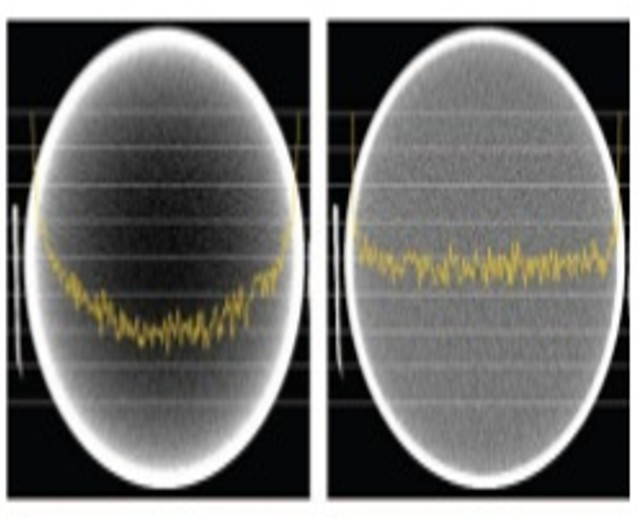
\includegraphics[width=\linewidth,keepaspectratio]{images/artefacto2.jpg}
%         \caption{Imagen 2}
%     \end{subfigure}

%     \vspace{3mm}

%     \begin{subfigure}[b]{0.38\textwidth}
%         \centering
%         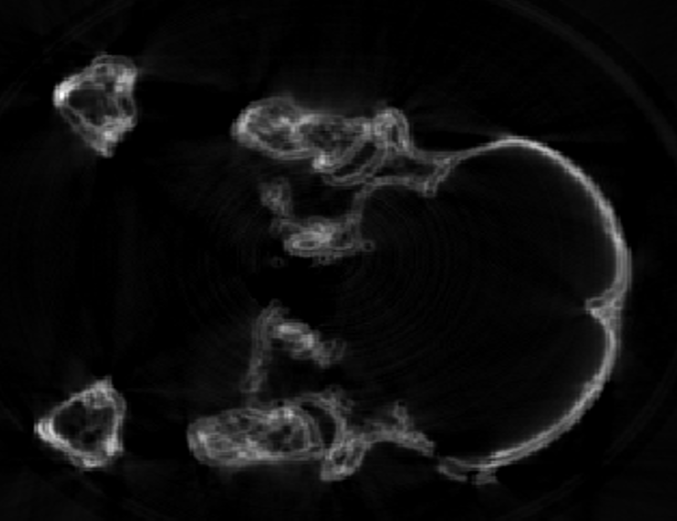
\includegraphics[width=\linewidth,keepaspectratio]{images/artefacto3.png}
%         \caption{Imagen 3}
%     \end{subfigure}
%     \hfill
%     \begin{subfigure}[b]{0.60\textwidth}
%         \centering
%         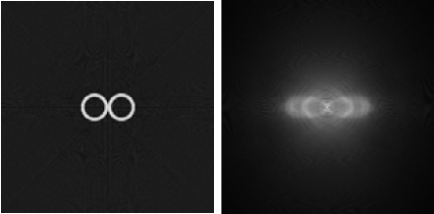
\includegraphics[width=\linewidth,keepaspectratio]{images/artefacto4.png}
%         \caption{Imagen 4}
%     \end{subfigure}
%     \caption{Algunos artefactos comunes en radiografías y tomografías. (a) Volumen parcial;
%     (b) y (c) endurecimiento del haz; (d) Movimientos del sistema/objeto; y (e) artefacto por
%     desalineación del sistema, en concreto, por una inclinación del detector.}
%     \label{fig:artefactos}
% \end{figure}

\begin{figure}[htpb]
    \centering
    \begin{subfigure}[b]{0.3\textwidth}
        \centering
        \begin{overpic}[width=\linewidth]{images/artefacto1.png}
            \put(3,70){\colorbox{black!60}{\color{white}\bfseries\large (a)}}
        \end{overpic}
    \end{subfigure}
    \hspace{2mm}
    \begin{subfigure}[b]{0.5\textwidth}
        \centering
        \begin{overpic}[width=\linewidth]{images/artefacto2.png}
            \put(3,40){\colorbox{black!60}{\color{white}\bfseries\large (b)}}
            \put(53,40){\colorbox{black!60}{\color{white}\bfseries\large (c)}}
        \end{overpic}
    \end{subfigure}

    \vspace{2mm}

    \begin{subfigure}[b]{0.3\textwidth}
        \centering
        \begin{overpic}[width=\linewidth]{images/artefacto3.png}
            \put(3,65){\colorbox{black!60}{\color{white}\bfseries\large (d)}}
        \end{overpic}
    \end{subfigure}
    \hspace{2mm}
    \begin{subfigure}[b]{0.50\textwidth}
        \centering
        \begin{overpic}[width=\linewidth]{images/artefacto4.png}
            \put(3,40){\colorbox{black!60}{\color{white}\bfseries\large (e)}}
            \put(53,40){\colorbox{black!60}{\color{white}\bfseries\large (f)}}
        \end{overpic}
    \end{subfigure}
    \caption{Algunos artefactos comunes en radiografías y tomografías. (a) Borde difuso por
    volumen parcial; (b) endurecimiento del haz en un cilindro homegéneo (c); (d) distorsiones
    en la imagen por movimientos del sistema/objeto;(e) es una imagen correspondiente a un
    sistema bien alineado, y (f) la misma imagen pero con un artefacto por
    desalineación del sistema, en concreto, por una inclinación del detector.}
    \label{fig:artefactos}
\end{figure}


\subsection{Una figura recurrente: la elipse}

Debido a la forma cónica del haz, y a las trayectorias circulares que realizan elementos
de la muestra durante la rotación, es común que las proyecciones radiográficas contengan
formas elípticas, por lo que es necesario tener en cuenta algunos conceptos útiles, tanto
para la alineación del sistema, como para el procesamiento digital.

Una elipse es una curva plana, simple y cerrada, que contiene puntos focales tales que,
para todos los puntos de la curva, la suma de las distancias a ambos focos es constante.
Es la generalización de la circunferencia, que es un tipo especial de elipse cuyos focos
coinciden en un mismo punto. Los diámetros más largo y más corto se denominan respectivamente,
el eje mayor (o \textit{ancho}) y el eje menor (o \textit{altura}), y se denotan por $2a$ y $2b$
(ver figura \ref{fig:elipse}.a). Los cuatro puntos de la curva que se ubican sobre estos ejes principales se conocen como 
\textit{vértices}. Una elipse cuyos ejes principales están alineados con los ejes $x$ e $y$,
centrada en el origen, puede describirse mediante la siguiente ecuación:

\begin{equation}
    \frac{x^2}{a^2} + \frac{y^2}{b^2} = 1
    \label{eq:elipse_simple}
\end{equation}

La elipse puede definirse también como una de las curvas cerradas (la otra es el
círculo) que se pueden formar en la intersección de un plano y la superficie de un cono
circular (ver \ref{fig:elipse}.b). Esta definición es particularmente útil para
microtomógrafos de haz cónico, en los que la pantalla del detector es el plano que interseca con
el cono. La ecuación que describe este tipo de curvas es $\hat{A}x^2 + \hat{B}xy +
\hat{C}y^2 + \hat{D}x + \hat{E}y + \hat{F} = 0$, con $\hat{B}^2 - 4\hat{A}\hat{C} < 0$, y puede ser reescrita
como

\begin{equation}
    A(x-x_0)^2 + B(y-y_0)^2 + 2C(x-x_0)(y-y_0) = 1
    \label{eq:elipse}
\end{equation}

\noindent donde $x_0$ e $y_0$ son las coordenadas del centro de la elipse, y $A$, $B$ y $C$ son
parámetros relacionados con el ancho, la altura y la orientación. En concreto, la misma ecuación
puede ser entendida como un producto matricial, entre $\mathbf{x}=(x-x_0, y-y_0)$ y una
matriz $\mathbb{A}$ que contiene toda la información de la elipse \cite{Strang2016}.

\begin{equation}
    \mathbf{x}^T \mathbb{A} \mathbf{x} = 1, \hspace{5mm} \mathbb{A} = \begin{bmatrix}
        A & C \\
        C & B
    \end{bmatrix}
    \label{eq:elipse_matriz}
\end{equation}

Al ser $\mathbb{A}$ una matriz real y simétrica, puede ser diagonalizada mediante una rotación.
Específicamente, si se rota el sistema de coordenadas hasta coincidir los ejes principales
de la elipse con los ejes cartesianos, entonces

\begin{equation}
    \mathbf{x'}^T 
    \begin{bmatrix}
        \lambda_1 & 0 \\
        0 & \lambda_2
    \end{bmatrix}
    \mathbf{x'} = 1 \hspace{5mm }\Longrightarrow \hspace{5mm} \lambda_1 x'^2 +  \lambda_2 y'^2 = 1
     \label{eq:elipse_diagonal}
\end{equation}

\noindent donde $\lambda_1$ y $\lambda_2$ son los autovalores de $\mathbb{A}$ y, a partir de la ecuación
\ref{eq:elipse_simple}, se puede deducir que $a = 1/\sqrt{\lambda_1}$ y $b = 1/\sqrt{\lambda_2}$.
Por otro lado, los autovectores de dicha matriz definen las direcciones de los ejes principales.
En concreto, si se toman las coordenadas del vector correspondiente al eje mayor, $\mathbf{v}_a=(v_{a,x},v_{a,y})$,
se puede obtener el ángulo de dicho eje con respecto a $x$, a través de la siguiente expresión \cite{Strang2016}.

\begin{equation}
    \theta = \arctan\left(\frac{v_{a,y}}{v_{a,x}}\right) = \frac{1}{2} \arctan\left(\frac{2C}{A-B}\right)
    \label{eq:angulo_elipse}
\end{equation}


\begin{figure}[htpb]
    \centering
    \begin{subfigure}{0.35\textwidth}
        \begin{overpic}
            [width=\textwidth]{images/general_ellipse.png}
            \put(3,95){\colorbox{black!60}{\color{white}\bfseries\large (a)}}
        \end{overpic}
        
    \end{subfigure}
    \hspace{10mm}
    \begin{subfigure}{0.35\textwidth}
        \begin{overpic}
            [width=\textwidth]{images/ellipse_conic.png}
            \put(3,95){\colorbox{black!60}{\color{white}\bfseries\large (b)}}
        \end{overpic}

    \end{subfigure}
    \caption{(a) Forma general de una elipse en el plano, definida por sus semi-ejes $a$ y $b$,
    su centro $(x_0,y_0)$ y su ángulo de inclinación $\theta$. (b) La elipse como producto de la intersección
    entre un plano y la superficie de un cono circular.}
    \label{fig:elipse}
\end{figure}

La ``elongación'' de una elipse se mide a través de la \textit{excentricidad}, que se calcula como

\begin{equation}
    e = \frac{c}{a} = \sqrt{1 - \frac{b^2}{a^2}}
    \label{eq:excentricidad}
\end{equation}

\noindent donde $c$ es la distancia entre el centro y uno de los focos. Para una circunferencia, $e=0$
y para una elipse $0<e<1$. Es de interés para este trabajo definir los siguientes criterios de evaluación de
``similitud'' entre una elipse y una circunferencia: la \textit{circularidad de Wadell} $C_W$ y
la \textit{relación de aspecto} $R$ (ambos menores a 1, e iguales solo en el caso de una
circunferencia), y el ángulo $\alpha$ entre los respectivas secciones cónicas.

\begin{equation}
    C_W = \frac{4\pi \cdot Area}{Perim^2} \hspace{10mm} R = \frac{b}{a}
    \label{eq:circ_R}
\end{equation}


Volviendo a la definición de la elipse como una sección cónica, se puede determinar el ángulo
de inclinación $\alpha'$ del plano de la elipse, con respecto al eje principal del cono, a partir
de los semi-ejes $a$ y $b$. La excentricidad de una sección cónica, producida por la
intersección de dicho plano, viene dada por $e=\cos\alpha'/\cos\beta$, donde $\beta$ el
semi-ángulo de apertura del cono. Luego, igualando con la ecuación \ref{eq:excentricidad}, 
y cambiando de variable a $\alpha = \pi/2 - \alpha'$, se obtiene la siguiente expresión:

\begin{equation}
    \alpha = \arcsin\left(\cos\beta \cdot \sqrt{1 - R^2}\right)
    \label{eq:alfa_proyeccion}
\end{equation}

\noindent donde el ángulo $\alpha$ es la inclinación del plano de la elipse con respecto a un plano
perpendicular al eje del cono (cuya sección cónica es una circunferencia), con el eje menor
como su eje de rotación \cite{Meserve1983} \cite{Larson2006}. Este último parámetro sirve también
para caracterizar la similitud de una elipse con un círculo (mientras más cercano a cero, más similar),
y será utilizado en el proceso de alineación.

\section{Procesamiento digital de imágenes}

En términos matemáticos, una imagen puede ser representada por medio de una función
bidimensional $f(x,y)$ donde las coordenadas $(x,y)$ (pixeles) se corresponden
con la posición en el plano, y el valor funcional indica la intensidad $I(x,y)$
en ese punto (ver figura \ref{fig:img_digital}). Existen dos tipos de imágenes comúnmente utilizadas: imágenes en
tonos de grises e imágenes a color, diferenciándose según cómo $f(x,y)$ representa
a la intensidad. En el primer caso, a cada pixel le corresponde un valor entero $g$
perteneciente a una escala entre 0 y $g_{max}=2^n -1$ ($2^n$ se corresponde con un formato
de ``n-bits'' para obtener dicha escala), tal que 0 representa al color negro y $2^n -1$ al blanco, y todo
tono de gris, un valor entre estos. En el segundo caso, la función $f(x,y)$ es un
vector de tres componentes (rojo, verde y azul), donde cada componente puede tomar
un valor entre 0 y $g_{max}$. Para una imagen radiográfica, la función $f(x,y)$ está
asociada directamente a la cantidad de fotones detectados en el foto-diodo $(x,y)$
del detector, una cantidad que es escalar para cada ``pixel'', por lo tanto, esta se
representa con tonos de grises. \cite{Martinsanz}\cite{Gonzalez}

\begin{figure}[htpb]
    \centering
    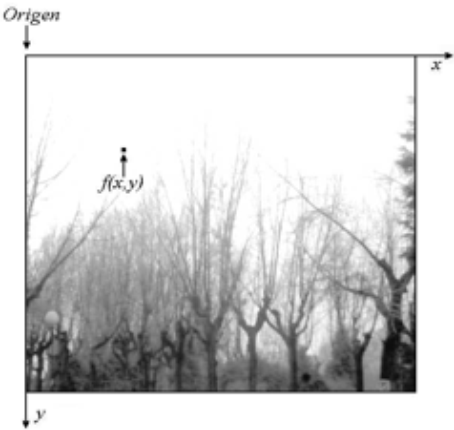
\includegraphics[width=0.45\textwidth]{images/img_digital.png}
    \caption{Representación matemática de una imagen digital. A cada pixel $(x,y)$ le
    corresponde un valor de intensidad dado por una función $f(x,y)$, escalar en el caso
    de tonos de gris, y vectorial en el caso de imágenes a color.}
    \label{fig:img_digital}
\end{figure}

\subsection{Conceptos estadísticos}

Una imagen típica puede contener millones de pixeles, sin embargo, sus valores de intensidad
no suelen ser totalmente aleatorios (para imágenes de objetos reales), por lo que es útil
analizarlos a partir de la estadística. A continuación, se definen algunos conceptos
estadísticos que se utilizaron en este trabajo.

\textit{Histograma} ($h(g)$):

El histograma de una imagen, o de una región de interés (ROI), es una función discreta que representa el número de
pixeles en la imagen en función de los niveles de grises $g$. $h(g)$ equivalente
a una distribución de probabilidad $P(g)$ de un determinado nivel de gris $g$.
Se define como

\begin{equation}
    h(g) = P(g) = n(g)/N 
    \label{eq:histograma}
\end{equation}

\noindent donde $n(g)$ es el número de pixeles con intensidad $g$, y $N$ es el número total
de pixeles en la imagen \cite{Martinsanz}. Al ser una distribución de probabilidad,
debe estar normalizada, es decir, $\sum_{g}h(g) = 1$. Esta función no brinda
información espacial, solo de la frecuencia de aparición de cada nivel de gris,
sin embargo, puede utilizarse para realizar segmentaciones. En la figura \ref{fig:histograma_ej}
puede encontrarse un ejemplo concreto.
\\

\begin{figure}[htpb]
    \centering
    \begin{subfigure}{0.35\textwidth}
        \begin{overpic}
            [width=\textwidth]{images/artefacto1.png}
            \put(2,74){\colorbox{black!60}{\color{white}\bfseries\large (a)}}
        \end{overpic}
        
    \end{subfigure}
    \hspace{10mm}
    \begin{subfigure}{0.40\textwidth}
        \begin{overpic}
            [width=\textwidth]{images/histograma_ej.png}
            \put(3,65){\colorbox{black!60}{\color{white}\bfseries\large (b)}}
        \end{overpic}

    \end{subfigure}
    \caption{Imagen de 632880 pixeles, en escala de grises 8-bit, con dos regiones bien marcadas
    (\textbf{a}) y su histograma (\textbf{b}).}
    \label{fig:histograma_ej}
\end{figure}

\textit{Valor Medio} ($VM$):

El valor medio de un ROI se define como el promedio de intensidades obtenidas,
y se calcula como

\begin{equation}
    VM = \langle I \rangle = \sum_{g=0}^{g_{max}}g\cdot h(g) = \sum_{x}\sum_{y}\frac{I(x,y)}{N}
    \label{eq:VM}
\end{equation}

\noindent donde $I(x,y)$ es la intensidad en el pixel $(x,y)$ \cite{Martinsanz}.
\\

\textit{Desviación Estándar (DS)}:

La $DS$ es una medida de dispersión de los valores de intensidad respecto al
valor medio, y se calcula mediante la siguiente expresión \cite{Martinsanz}

\begin{equation}
    DS^2 = \sum_{g=0}^{g_{max}}(g-VM)^2h(g) = \sum_{x}\sum_{y}\frac{(I(x,y)-VM)^2}{N}
    \label{eq:DS}
\end{equation}\\

\textit{Relación Señal Ruido (SNR)}:

Relación entre la señal (representada por $I$, el número de fotones detectados)
y el ruido estadístico asociado al proceso de adquisición $\sigma$
\cite{Martinsanz} \cite{Gonzalez}. Se considera como SNR de un ROI el valor medio
de los SNR de todos los pixeles del ROI.

\begin{equation}
    SNR = \left\langle \frac{I(x,y)}{\sigma} \right\rangle
    \label{eq:SNR}
\end{equation}

Cuando el $SNR$ toma valores pequeños, el ruido estadístico es comparable con la
intensidad detectada (ver figura \ref{fig:SNR}). El criterio de Rose afirma que para poder distinguir las
características de la imagen con 100$\%$ de certeza es necesario que el $SNR$
tome valores mayores a 5 \cite{Bushberg}.\\

\begin{figure}[htpb]
    \centering
    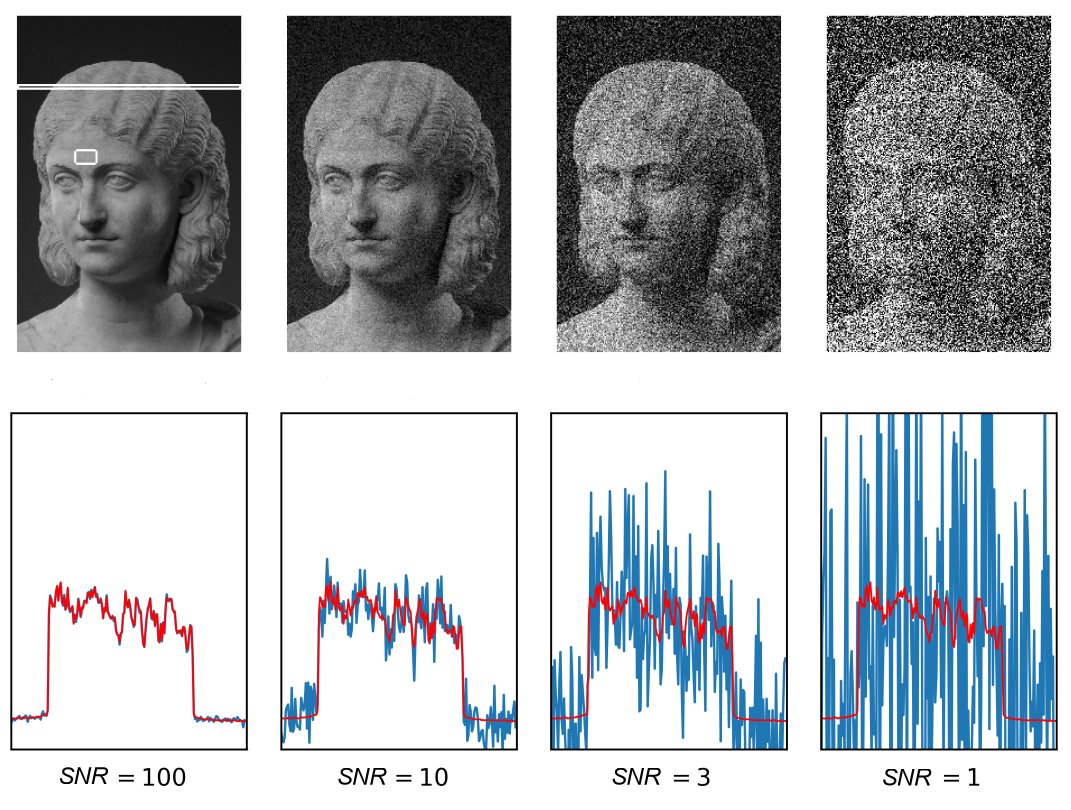
\includegraphics[width=0.70\textwidth]{images/SNR.png}
    \caption{Visualización de distintos niveles de $SNR$ para una misma imagen.}
    \label{fig:SNR}
\end{figure}

\textit{Relación Constraste Ruido (CNR):}

Se define el $CNR$ entre los puntos A y B de un ROI como el contraste de
intensidades entre dichos puntos $I_A - I_B$ sobre el ruido estadístico asociado
al proceso de adquisición $\sigma$ \cite{Bushberg}. Representa la
capacidad de distinguir la variación de intensidades entre las dos regiones de
la imagen.

\begin{equation}
    CNR = \frac{I_A - I_B}{\sigma}
    \label{eq:CNR}
\end{equation}

\subsection{Transformaciones Geométricas}

El análisis y la corrección de desalineaciones de un microtomógrafo requiere saber cómo se
puede transformar una imagen al considerarla como un elemento geométrico. Una 
transformación geométrica de una imagen es una operación que redefine la
disposición espacial de los datos sin alterar (idealmente) la naturaleza de la
información capturada. Estas transformaciones pueden describirse según qué propiedades del objeto original
preservan. Algunos ejemplos pertinentes para este trabajo son los siguientes (ver
figura \ref{fig:transformaciones}).

\begin{enumerate}[label=\alph*)]
    \item \textit{Isometrías}: Preservan distancias y ángulos (rotación y traslación).
    \item \textit{Similitudes}: Preservan la forma pero cambian el tamaño (escalado).
    \item \textit{Afines}: Preservan el paralelismo (shear).
    \item \textit{Proyectivas}: No preservan ángulos ni paralelismo; solo preservan la
    colinealidad (cambios de perspectiva).
\end{enumerate}

\begin{figure}[htpb]
    \centering
    \begin{subfigure}{0.25\textwidth}
        \begin{overpic}
            [width=\textwidth]{images/normal_im.png}
            \put(3,82){\colorbox{black!60}{\color{white}\bfseries\large (a)}}
        \end{overpic}
    \end{subfigure}
    \hspace{3mm}
    \begin{subfigure}{0.25\textwidth}
        \begin{overpic}
            [width=\textwidth]{images/rotation.png}
            \put(3,82){\colorbox{black!60}{\color{white}\bfseries\large (b)}}
        \end{overpic}
    \end{subfigure}
    \hspace{3mm}
    \begin{subfigure}{0.25\textwidth}
        \begin{overpic}
            [width=\textwidth]{images/translation.png}
            \put(3,82){\colorbox{black!60}{\color{white}\bfseries\large (c)}}
        \end{overpic}
    \end{subfigure}
    \vspace{2mm}
    \begin{subfigure}{0.25\textwidth}
        \begin{overpic}
            [width=\textwidth]{images/scale.png}
            \put(3,82){\colorbox{black!60}{\color{white}\bfseries\large (d)}}
        \end{overpic}
    \end{subfigure}
    \hspace{3mm}
    \begin{subfigure}{0.25\textwidth}
        \begin{overpic}
            [width=\textwidth]{images/shear.png}
            \put(3,82){\colorbox{black!60}{\color{white}\bfseries\large (e)}}
        \end{overpic}
    \end{subfigure}
    \hspace{3mm}
    \begin{subfigure}{0.25\textwidth}
        \begin{overpic}
            [width=\textwidth]{images/projective.png}
            \put(3,82){\colorbox{black!60}{\color{white}\bfseries\large (f)}}
        \end{overpic}
    \end{subfigure}
    \caption{Algunas de las principales transformaciones geométricas de una imagen.
    (a) Imagen original. (b) Rotación isométrica afín. (c) Traslación isométrica afín.
    (d) Escalado. (e) Shear. (f) Cambio de perspectiva (proyección).}
    \label{fig:transformaciones}
\end{figure}

En términos matemáticos, si una imagen es una función
$f(\mathbf{x})$ que asigna un número (tonalidad de gris) a un vector (pixel) $\mathbf{x} = (x,y)$,
entonces una transformación geométrica es un mapeo de la forma $g(\mathbf{x'})=
f(T^{-1}(\mathbf{x'}))$ donde $T$ es la función de transformación que mapea las
coordenadas originales a las nuevas, es decir, $\mathbf{x'}=T(\mathbf{x})$; y $g(\mathbf{x'})$
es la intensidad que debe conservarse en la transformación al nuevo sistema. 

Para facilitar el cálculo computacional, el mapeo espacial se realiza mediante
productos de matrices, utilizando las \textit{coordenadas homogéneas} $\mathbf{X}$
y $\mathbf{X'}$  (que agregan una dimensión a los vectores $\mathbf{x}$ y
$\mathbf{x'}$) \cite{Rhody2005}, de forma tal que cualquier transformación puede expresarse como

\begin{equation}
    \mathbf{X'}=\mathbb{H}\mathbf{X}
    \longrightarrow
    \begin{pmatrix}
        X' \\
        Y' \\
        W'
    \end{pmatrix}
    =
    \begin{pmatrix}
        r_{11} & r_{12} & t_x \\
        r_{21} & r_{22} & t_y \\
        g & h & 1
    \end{pmatrix}
    \begin{pmatrix}
        x \\
        y \\
        1
    \end{pmatrix}
    \label{eq:coord_homog}
\end{equation}

\noindent donde $\mathbb{H}$ es la matriz de transformación (general); la submatriz $2\times
2$ de elementos $r_{ij}$ controla las rotaciones y escalado; el vector columna
$(t_x, t_y)$ controla las traslaciones; y el vector fila $(g,h)$ controla la
proyección. Por otro lado, la nueva coordenada $W'$ es un factor de escala en
el nuevo sistema de coordenadas, de forma tal que las coordenadas de la imagen
real (transformada) son $x'=X'/W'$ e $y'=Y'/W'$, y este es distinto de 1 solo
cuando la transformación es proyectiva ($g\neq 0$ o $h\neq 0$). Una transformación
arbitraria puede ser entendida como una composición de las transformaciones básicas, y
matemáticamente, como un producto de matrices $\mathbb{H} = \mathbb{H}_n \cdot \mathbb{H}_{n-1}
\cdot ... \cdot \mathbb{H}_1$, donde el orden de las transformaciones es importante,
ya que el producto de matrices no es conmutativo. \cite{Rhody2005}

Por otro lado, en una imagen real, la función $f(x,y)$ toma vectores discretos de una grilla,
por lo que generalmente el mapeo inverso suele resultar en coordenadas no enteras
(por ejemplo al rotar una imagen, como se observa en la figura \ref{fig:transformaciones}).
Para solucionar esto, toda operación de transformación implica también una
estimación de intensidad de los pixeles nuevos, que se realiza a través de una
interpolación. Debido a esto, obtener una imagen tomográfica fiel no se consigue
simplemente conociendo las desalineaciones y corrigiéndolas a partir de la ecuación
\ref{eq:coord_homog}, sino buscando reducirlas al mínimo posible, para evitar
múltiples interpolaciones.

\subsection{Segmentación}

Otra técnica útil que se utilizó a lo largo de este trabajo, para procesar imágenes
que tengan estructuras con intensidades bien definidas y distinguibles entre sí, es la
\textit{segmentación}. Esta se define como la operación de \textit{etiquetar pixeles que posean
ciertas características}, y destacarlos de aquellos que no las posean. Los métodos
de segmentación son muchos y variados, según la finalidad y la forma de operar. Sin
embargo, para este trabajo se utilizará uno de los más básicos, la segmentación
por \textit{umbralización}, basada en similitudes entre pixeles.

La umbralización es una técnica muy utilizada en la detección de objetos, consiste
en aplicar una transformación $T$ en los valores de la intensidad $I(x,y)$, obteniendo
como resultante una imagen binaria $B(x,y)=T[I(x,y)]$, que toma valores iguales a 1 en
las coordenadas donde la imagen original posee valores mayores a un cierto umbral $t$,
y a cero en el caso contrario. En una imagen radiográfica, en general se
desea distinguir objetos (más absorbentes) de un fondo (menos absorbente), por lo
que se buscaría un umbral tal que la función binaria $B(x,y)$ solo tome valores
distintos de cero fuera del objeto (ver figura \ref{fig:umbralizacion}).

\begin{equation}
    B(x,y)=
    \begin{cases}
        0 & I(x,y)<t\\
        1 & I(x,y)\geq t
    \end{cases}
    \label{eq:umbralización}
\end{equation}

Si una imagen presenta objetos de distinta naturaleza (con distintos niveles de grises),
puede emplearse un umbral superior y uno inferior, $t_{max}$ y $t_{min}$ respectivamente,
tal que $B(x,y)$ resalte solo los pixeles que cumplan $t_{min}<I(x,y)<t_{max}$. De
esta forma, aplicando distintos rangos de umbrales, se puede segmentar cada tipo
de objeto con mayor precisión.

\begin{figure}[htpb]
    \centering
    \begin{subfigure}{0.35\textwidth}
        \begin{overpic}
            [width=\textwidth]{images/esferas_yang.png}
            \put(2,70){\colorbox{black!60}{\color{white}\bfseries\large (a)}}
        \end{overpic}
        
    \end{subfigure}
    \hspace{5mm}
    \begin{subfigure}{0.35\textwidth}
        \begin{overpic}
            [width=\textwidth]{images/esferas_yang_umbral.png}
            \put(3,70){\colorbox{black!60}{\color{white}\bfseries\large (b)}}
        \end{overpic}

    \end{subfigure}
    \caption{(\textbf{a}) Proyección radiográfica de un cilindro de acrílico con esferas metálicas
    incrustadas en su superficie. (\textbf{b}) Segmentación de las esferas a partir de una umbralización.}
    \label{fig:umbralizacion}
\end{figure}
